%% JSSAM (OUP) submission, double-blind: authorship and funding live on
%% titlepage.tex, not here. v10: full narrative restructure of the frozen
%% v9/v8.2 results around the recording-pipeline boundary. Every retained
%% number traces to artifact/claim_manifest.csv or to the exploratory Build
%% geo15 outputs (RESULT_PROVENANCE.md); no result of a pre-registered
%% analysis is altered. New exploratory L1/L3 work is labeled as such.
\documentclass[12pt]{article}
\usepackage[margin=1in]{geometry}
\usepackage{amsmath}
\usepackage{amssymb}
\usepackage{graphicx}
\usepackage{booktabs}
\usepackage{natbib}   %% ASA author-date (JSSAM)
\setcitestyle{round,aysep={}}
\usepackage{url}

\graphicspath{{figures_v10/}}
\newcommand{\keff}{k_{\mathrm{eff}}}
\newcommand{\rmass}{\rho}

\title{When Numerical Structure Reads the Recording Pipeline:\\
A Boundary for Factorization-Based Data Analysis}
\author{}   %% BLINDED for double-blind review --- authorship on titlepage.tex
\date{}

\begin{document}
\maketitle

\begin{abstract}
Digit-based forensic tests are increasingly run against published official
statistics, where an extreme test statistic may reflect how the values were
recorded rather than how they were generated. In a real case, a standard
election-forensics last-digit test fires catastrophically
($\chi^2_9 = 12{,}684$) on the Census Bureau's citizen-voting-age-population
tabulation---a modeled series published on a five-unit rounding grid---while
genuine enumerated returns pass. The test cannot distinguish fabrication
from a documented publication rule. We present a small set of integer-arithmetic \emph{recording-grid
coordinates} that identify such alarms as grid-compatible---and, where the
recording rule is documented, attribute them to it---demonstrated here and in a second
case localizing a survey publication grid to its margin-of-error column. The design follows from the paper's central result:
within the recorded-data classes tested, and under stated recording
assumptions, factorization \emph{shape}---what a value's prime factorization
looks like once prime names are discarded---retains only the value's
magnitude and its most recent recording or quantizing operation, not its deeper
generating history. Across roughly 19{,}000 integer channels, all apparent shape structure
reduces to four drivers (magnitude, decimal rounding, small-prime
composition, residue quantization); grouped held-out analysis shows the
apparent shape geography carries essentially no process information beyond
recording variables. The boundary is mechanistic---one added unit destroys the
multiplicative-construction signal---and powered: a host-matched
quotient-level alternative is recovered at a $5\%$ mixture in six of six
channels. Exact, unrounded
multiplicative integers remain a positive regime. The practical warning for
official-statistics users, forensic analysts, and auditors: a detector firing
on a recorded number does not establish that it read the underlying activity;
it may have read the last recording operation. All confirmatory claims were prospectively specified in internally frozen
analysis plans; three missed their frozen rules and are reported.
\end{abstract}

\medskip
\noindent\textbf{Keywords:} data quality; data provenance; digit analysis;
rounding; heaping; quantization; prime factorization; election forensics;
pre-registration

\medskip
\noindent\textbf{Statement of Significance.}
Analysts screen published statistics---population tabulations, employment
series, survey margins of error---with digit-based tests for signs of
fabrication or error. This paper documents, on real federal statistical
products, how badly such a screen can mislead: a standard forensic test
declares an extreme anomaly on an ordinary Census tabulation whose only
peculiarity is that the agency rounds published values to the nearest five.
We provide a simple set of arithmetic measurements, computed from the published
integers alone, that identify when an alarm is explained by such a recording
rule, and we establish---with prospectively specified analyses across roughly
19{,}000 data columns---why this works: in the data classes tested, after ordinary recording (summing, counting,
rounding), the arithmetic fine structure of a number retains the recording
rule and essentially nothing else about how the quantity arose. The result
protects data users from a documented class of false accusations, and warns
that statistical extremity alone does not license conclusions about data
integrity.

\section{A false alarm on a published statistic}
\label{sec:vignette}

An analyst screening turnout-related integer series for irregularities will
sooner or later apply a last-digit uniformity test~\citep{beberscacco2012} to
the U.S.\ Census Bureau's citizen-voting-age-population (CVAP) tabulation---a
natural denominator for turnout~\citep{censuscvap2022}. On county-level values
of at least $1000$ (the test's standard magnitude screen), the test statistic
is $\chi^2_9 = 12{,}684$ ($p$ below reporting precision): among the most
extreme digit
anomalies one can observe on a published series. Run beside it, genuine
certified election returns pass comfortably---North Carolina precinct returns
and nationwide county returns for two presidential elections give
$p \ge 0.16$~\citep{ncsbe,countyreturns}. Figure~\ref{fig:cvap} shows what the
test saw: nearly all CVAP values end in $0$ or $5$.

\begin{figure}[!htb]
\centering
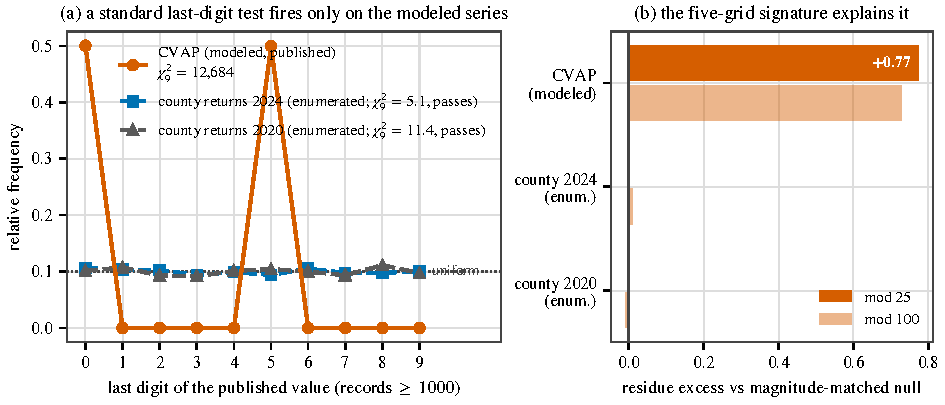
\includegraphics[width=\linewidth]{fig1_cvap_false_alarm}
\caption{The CVAP false alarm and its attribution. (a)~Last-digit
distributions on records $\ge 1000$: the modeled CVAP series concentrates on
terminal $0$ and $5$ and fires the Beber--Scacco test at
$\chi^2_9=12{,}684$; enumerated county returns are uniform and pass. (b)~The
recording-grid coordinates identify the alarm as grid-compatible: CVAP's
residue distribution modulo $25$ (and $100$) departs from the
magnitude-matched uniform reference by $+0.77$ ($+0.73$), the direct
signature of rounding to the nearest five; every enumerated series is at
zero. The Bureau's documented nearest-five rule completes the attribution.}
\label{fig:cvap}
\end{figure}

The alarm is real; the natural interpretation is wrong. CVAP is not an
enumerated count. It is an American Community Survey special tabulation---a
\emph{modeled estimate}---and the Bureau publishes it rounded to the nearest
five~\citep{censuscvap2022,cvaptechdoc}. A five-grid forces terminal digits into
$\{0,5\}$; the test fires on the publication rule. The test statistic cannot
know that: last-digit uniformity is a valid fabrication screen only under
assumptions about how the values were generated \emph{and recorded}, and a
publication grid violates them innocently. The coordinates in
Figure~\ref{fig:cvap}(b), computed from the published integers alone, supply
the missing step: the residue distribution of the CVAP values modulo $25$
exceeds a magnitude-matched uniform reference by $+0.77$ in total
variation---the arithmetic fingerprint of a five-grid---while every
enumerated series carries none; the Bureau's documented rounding rule then
completes the attribution. The correct disposition is ``recording
artifact,'' not ``irregularity.''

Three scope statements, made once. CVAP is a modeled published series, not a
vote count. The analysis throughout is methodological---about recording rules
and the reading of digit-forensic alarms---and makes no claim about the
legitimacy of any election. And the case does not show that forensic alarms
are generally innocent; it shows that an alarm cannot be interpreted until the
recording process has been considered.

\section{Research question and contributions}
\label{sec:question}

The CVAP case poses the question this paper answers: \emph{when a statistical
detector fires on a recorded number, what did it actually read---the
generating process, or the way the values were recorded?}

We answer it for one family of representations: integer factorization. Every
integer's prime factorization is a complete invariant, and it is natural to
hope that a fine arithmetic lens might read provenance---whether a value was
built by multiplication, counting, or estimation---directly off stored data.
Data-quality practice already reads coarser projections of the same digits:
leading-digit conformance tests~\citep{benford1938,hill1995,nigrini2012},
last-digit and duplication screens~\citep{beberscacco2012}, heaping
indices~\citep{myers1940,whipple1919,ahearn2009}, and price-clustering
diagnostics~\citep{harris1991}. The paper makes three contributions, and no
more:

\begin{enumerate}
\item \textbf{A conditional boundary} on what factorization shape retains in
recorded administrative data: within the recorded-data classes tested, and
under the recording assumptions stated in Section~\ref{sec:model},
factorization shape reflects magnitude and the most recent recording or
quantizing operation---not deeper generating history
(Sections~\ref{sec:geography}--\ref{sec:drivers}).
\item \textbf{A powered, mechanistically supported explanation} for the
boundary: one additive unit destroys the multiplicative-construction signal,
and the pipeline demonstrably recovers a matched surviving alternative at a
$5\%$ mixture, so the negative is not underpowered
(Sections~\ref{sec:mechanism}--\ref{sec:power}).
\item \textbf{A narrow recording-grid attribution instrument}, predicted by
the boundary (if the grid is what survives, measure the grid), demonstrated in
two real cases---the CVAP false alarm above and an ACS margin-of-error
localization---that prevents a demonstrated class of grid-induced forensic
false interpretations (the gate's own output is ``grid-compatible'';
attribution is claimed only where the recording rule is documented)
(Section~\ref{sec:instrument}).
\end{enumerate}

The instrument's demonstrated real-data role is attribution in two cases, not
general fabrication detection; on real returns it does not outperform
established digit tests as a detector, and we say so where the comparison is
made. Digit-based tests are treated throughout as complementary projections
with their own assumptions, not as inferior methods.

\section{A minimal model of representation and recording}
\label{sec:model}

Four objects carry the whole argument; everything else (algorithms, null
construction, finite-size detail) is in the supplement.

\paragraph{Factorization shape: the L-profile.}
For an integer $n = \prod_{i=1}^{r} p_i^{a_i}$, each prime-power part
contributes $a_i \ln p_i$ of the value's log-magnitude. Normalizing and
sorting gives the \emph{L-profile}
\begin{equation}
\ell_j = \frac{a_{(j)} \ln p_{(j)}}{\ln n}, \qquad
\ell_1 \ge \ell_2 \ge \cdots \ge \ell_r, \qquad \textstyle\sum_j \ell_j = 1,
\label{eq:lprofile}
\end{equation}
from which we read $L_1 = \ell_1$, $L_3 = \ell_3$,
$\mathrm{Tail} = 1 - \ell_1 - \ell_2$, and the concentration
$H_2 = \sum_j \ell_j^2$. The profile is a \emph{shape} object: it records how
log-magnitude is spread across multiplicative parts. Every claim in this
paper about ``shape'' concerns functionals of the log-share multiset
$\{a_i \ln p_i\}$---blind to prime \emph{names} given their sizes, though
not to the sizes themselves (small primes carry small log-shares, which is
what makes driver 3 of Section~\ref{sec:drivers} visible). Shape is
deliberately distinguished from \emph{named-prime} instruments: a readout
keyed to particular primes (say, the factor $5$ a rounding rule injects) is a
different projection with a different boundary, and the attribution
instrument below is prime-aware by design.

\paragraph{The magnitude-conditioned baseline.}
The reference for shape is the behavior of uniform random integers. Their
normalized factor sizes converge to the Poisson--Dirichlet
law~\citep{billingsley1972,kingman1975,arratia2000}, with
$\mathbb{E}[L_1] \to 0.6243$, but convergence is far too slow for real data:
$\mathbb{E}[L_1 \mid d]$ falls from $0.952$ for $1$-digit integers to $0.633$
at $18$ digits (a Dickman-type computation~\citep{dickman1930}). Magnitude
alone therefore moves the profile more than any effect studied below, and all
structural claims are residuals against this \emph{magnitude-conditioned
baseline} $\mathbb{E}[\,\cdot \mid d\,]$, with $d$ the digit length. The
channel-level summary is a ratio of averages,
\begin{equation}
\keff \;=\; \frac{\sum_d w_d\, \mathbb{E}[H_2 \mid d]}{\overline{H_2}},
\label{eq:keff}
\end{equation}
with $w_d$ the channel's digit histogram and $\overline{H_2}$ its mean
concentration over records (records with fewer than three prime-power parts
contribute their exact $H_2$; the structural-zero treatment of $L_3$ is in
Section~\ref{sec:geography}). It equals $1$ for generic integers, exceeds
$1$ when multiplicative energy spreads across more parts than chance, and
falls below $1$ for concentration.

\paragraph{The recording-grid coordinates.}
Where the L-profile is blind to prime names, the attribution instrument reads exactly
the primes and residues a recording rule injects: the \emph{grid mass}
$\rmass$ (the log-share of a value carried by the primes $2$ and $5$, split
into its $2$- and $5$-components), the \emph{grid depth} (the power of ten
dividing the value), \emph{grid conformance} (the fraction of records on the
channel's modal grid), and \emph{residue quantization} $Q_m$ (the
total-variation distance of values modulo $m$ from uniform, scored against a
magnitude-matched reference, at moduli such as $25$, $49$, $47$, $43$). All
are computed from stored integers alone; a units change (dollars to cents)
shifts $\rmass$ predictably and leaves the residual coordinates invariant. The
supplement gives the full definitions and the channel-level algorithm.

\paragraph{The recording model, and the shape window.}
A recorded integer is modeled as
\begin{equation}
n = g \cdot q, \qquad g = 2^{s} 5^{t} m_0, \qquad
q = \mathrm{round}(x / g),
\label{eq:pipeline}
\end{equation}
where $x$ is the latent quantity, $g$ is the recording grid (a decimal grid,
optionally times a non-decimal tick $m_0$), and $q$ is the stored quotient.
A publication grid is one kind of recording rule; the model covers any rule
whose last operation multiplies a generic quotient by a fixed factor.
Under one modeling assumption---\emph{local flatness}, that the pre-rounding
density of $x/g$ is roughly constant across one grid cell---the quotient $q$
is, to first order, a generic integer: its factorization carries no imprint of
the process that produced $x$. Equation~\eqref{eq:pipeline} then fixes the
division of labor. The shape of $n$ is the shape of $g \cdot q$; since $q$ is
generic, all non-magnitude shape structure comes from $g$. The grid mass and
depth read the decimal part of $g$; the residue coordinates read a non-decimal
tick $m_0$ that leaves no trace in terminal digits. We call the multiplicative
structure a value retains its \emph{shape window}: \textbf{the accumulated
multiplicative history since the last additive or quantizing operation applied
to the value}. For an exact product never subsequently summed or rounded, the
window contains the whole construction. For an ordinary recorded value, the
model predicts the window contains the grid and nothing else.

\paragraph{Scope, stated once.}
Two qualifications govern everything that follows. First, the genericity of
$q$ rests on local flatness and on the near-independence of the factorizations
of consecutive integers; the latter is a heuristic---the exact statement is a
Chowla-type correlation problem, open in
general~\citep{taoteravainen2019}---so the boundary is a
\emph{conditional empirical claim}, not a theorem. Second, the completeness of
the four-driver reduction below is an empirical finding in the tested corpus,
consistent with the model's prediction, not a proof that no fifth driver
exists. The claims are scoped to shape functionals of the log-share multiset
$\{a_i \ln p_i\}$ (blind to prime names given their sizes), on the
recorded-data classes tested, under model~\eqref{eq:pipeline}.

\section{The apparent geography}
\label{sec:geography}

Suppose an analyst suspects that integer fields of different provenance carry
different multiplicative character, and maps a large corpus of fields by their
factorization shape. We ran exactly this. The corpus is $18{,}951$ integer
%

channels (one integer-valued column of one dataset, deduplicated by content
fingerprint) in $367$ dataset-families across $18$ domains---equity markets, census,
network telemetry, procurement, seismology, real estate, health, and
others---with ${\sim}9.6\times10^{8}$ exact factorizations
(Table~\ref{tab:corpus}; construction details in the supplement; the
``roughly 19{,}000'' used elsewhere rounds this frozen count, and the
supplement's \S S4 footnote reconciles the two related profile-set counts).
The \texttt{unresolved} row collects channels whose domain the frozen
labeling rules could not assign; they are excluded from every domain-labeled
analysis. Channel
counts are dominated by a few high-volume administrative sources, a property
the reader needs when judging the scope of every claim below.

\begin{table}[t]
\centering
\caption{Corpus composition (frozen post-quarantine set: $18{,}951$ channels,
$367$ dataset-families, $18$ domain labels).}
\label{tab:corpus}
\small
\begin{tabular}{lrr@{\hskip 2em}lrr}
\toprule
domain & channels & families & domain & channels & families \\
\midrule
network\_telemetry   & 14{,}929 & 6   & seismology      & 84 & 34 \\
procurement          & 1{,}812  & 8   & payments\_fraud & 77 & 11 \\
census               & 1{,}105  & 26  & sports          & 77 & 13 \\
unresolved           & 159      & 79  & real\_estate    & 55 & 12 \\
equity\_markets      & 146      & 103 & food\_nutrition & 27 & 10 \\
campaign\_finance    & 137      & 3   & genomics        & 13 & 11 \\
health               & 115      & 8   & crime           & 11 & 3  \\
admin\_codes         & 102      & 3   & accounting      & 10 & 4  \\
corporate\_financials& 90       & 32  & taxi\_trips     & 2  & 1  \\
\bottomrule
\end{tabular}
\end{table}

The map looks like a discovery. In the raw $(L_1, \mathrm{Tail})$ plane the
$367$ families form three clean, reproducible clusters (silhouette $0.719$);
in the raw $(L_1, L_3)$ plane of Figure~\ref{fig:geography}(a) the channels
trace a structured band with a prominent arm. A shape-based provenance
taxonomy---``these fields are multiplicative, those are counts, those are
prices''---appears within reach.

\begin{figure}[t]
\centering
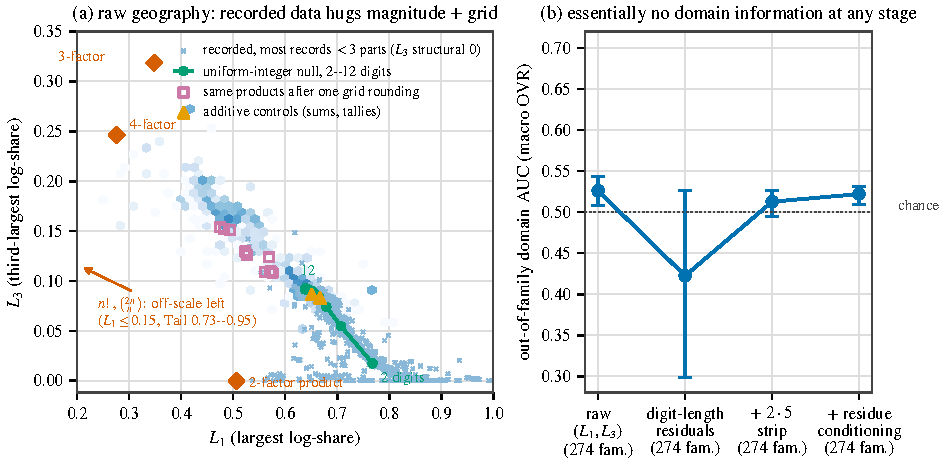
\includegraphics[width=\linewidth]{fig2_geography_raw_controlled}
\caption{The apparent geography and what it maps. (a)~Channel-level
$(L_1, L_3)$ plane: recorded channels (blue density; crosses mark channels
whose records mostly have fewer than three prime-power parts, for which $L_3$
is structurally zero) hug the magnitude-conditioned baseline curve (green:
uniform-integer pseudo-channels, $2$--$12$ digits) extended by a
decimal-rounding arm. Exact multiplicative constructions (red diamonds) sit
far off the band---and land back on it after a single decimal-grid rounding
(open squares). Additive controls (sums, tallies; orange) sit exactly on the
baseline. (b)~Out-of-family domain information in the coordinates at each
control stage (grouped $5$-fold by dataset-family, macro one-vs-rest AUC,
family-bootstrap $90\%$ intervals): the map's visible structure carries
essentially no cross-source process information even before controls.
Exploratory analysis (Build geo15).}
\label{fig:geography}
\end{figure}

Figure~\ref{fig:geography}(a) already contains the refutation, because every
comparator on the map is matched. The uniform-integer baseline traces exactly
the band's spine: position along the band is magnitude. The arm is decimal
rounding: exact products relocated onto the arm by a single grid rounding sit
among the recorded channels. Additive controls are indistinguishable from the
baseline. The only points far from the band are exact multiplicative
constructions that no recording operation has touched. (One representational
caveat is marked explicitly: $37.5\%$ of sampled records have fewer than three
prime-power parts, so per-record $L_3$ is a structural zero, not a small
continuous value; channels dominated by such records are faceted separately,
and the supplement gives the per-record analysis.)

Two quantitative results close the case against the taxonomy reading. First,
the frozen corpus analyses showed the three clusters are ordered segments of a
single variable---the grid mass $\rmass$---and dissolve when the decimal
primes are divided out (cluster survival Jaccard $0.39$--$0.43$); a supervised
``domain signal'' on monetary channels reverses sign under a units change
(cents versus dollars), exposing it as a scale artifact; and the cleaned space
is a one-dimensional magnitude continuum (intrinsic dimension $1.16$ by the
TwoNN estimator~\citep{facco2017}) with no
domain islands. Second---new in this version, and exploratory---a grouped
transfer test asks whether the coordinates carry \emph{any} domain information
across independent dataset-families: predicting a channel's domain from its
raw $(L_1, L_3)$ position, with entire families held out, achieves macro AUC
$0.526$ ($90\%$ CI $[0.508, 0.543]$: above $0.5$, but weak and practically
negligible), and no stage restores it
(Figure~\ref{fig:geography}(b)). A positive control calibrates the design's
sensitivity: the identical family-grouped pipeline reads synthetic recording
differences at AUC $0.81$ for a grid-mass shift of $+0.020$ and $0.99$ at
$+0.066$, with a family-permutation null centered at $0.485$ (supplement
\S S4). The transfer information the real coordinates carry is
therefore an order of magnitude below what a modest recording difference
produces. The apparent geography was never a usable process taxonomy, even
before controls: it is a map of magnitude and recording, mistaken for one
because magnitude and recording conventions correlate with domains within
any fixed corpus.

\section{The four-driver reduction}
\label{sec:drivers}

The claim that the map is ``magnitude and recording'' is made precise by an
explicit reduction. The full distributional deviation of each channel's
profile from the magnitude-conditioned baseline---measured by Wasserstein and
energy distances, so the whole shape is compared, not two summary
moments---is attributed hierarchically to four drivers, each with a removal
operator (Table~\ref{tab:decomp}).

\begin{table}[t]
\centering
\caption{The four-driver reduction: each driver of raw shape structure, its
effect, and the operator that removes it. After all four, no shape structure
remains (the surviving candidate collapses under its own control,
Figure~\ref{fig:waterfall}).}
\label{tab:decomp}
\small
\begin{tabular}{p{0.24\linewidth}p{0.40\linewidth}p{0.26\linewidth}}
\toprule
driver & effect & removal operator \\
\midrule
1. magnitude (digit length) & dominant; raw map tracks the baseline curve & magnitude-conditioned baseline $\mathbb{E}[\cdot\mid d]$ \\
2. decimal rounding ($2\cdot5$) & the entire raw arm; Tail excess up to $+0.11$ & divide out $2^{v_2}5^{v_5}$, re-baseline the core \\
3. small-prime composition ($3, 7$; $11, 13$ via the $\le13$ strip; $2, 5$ belong to driver 2) & $25$--$50\%$ of the de-rounded overshoot & strip primes $\le 7$, $\le 13$ \\
4. residue quantization (ticks, grids) & incremental $\Delta R^2 = +0.043$; partial correlation $r = 0.488$ & residue scores $Q_m$, negative-controlled \\
\midrule
\emph{(surviving candidate)} & concentration excess $-0.0184$ & core-magnitude re-indexing $\to -0.0001$ \\
\bottomrule
\end{tabular}
\end{table}

\begin{figure}[t]
\centering
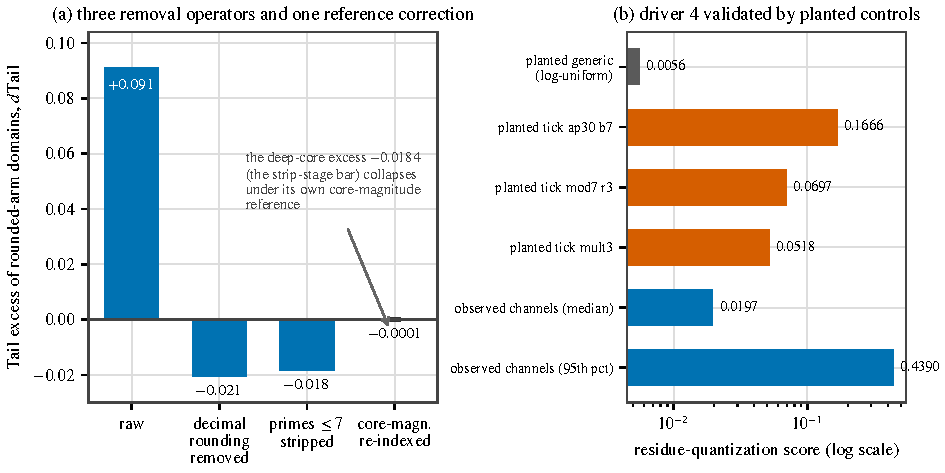
\includegraphics[width=\linewidth]{fig3_driver_waterfall}
\caption{Driver removal. (a)~Tail excess of the frozen arm domains at
family-equal weighting (the same estimand as the leave-one-source-out
analysis, supplement \S S3): raw (driver 1 removed by the baseline), after
dividing out decimal rounding (driver 2), after stripping primes $\le 7$
(driver 3)---this strip-stage value \emph{is} the deep-core concentration
excess $-0.0184$---and after core-magnitude re-indexing, the reference
correction under which it collapses to $-0.0001$ ($90\%$ family-bootstrap
CI $[-0.0004, +0.0004]$). (b)~Driver 4
validated by planted negative controls: channels quantized onto ticks score
$10$--$30\times$ above planted generic (log-uniform) channels on the residue
score; observed channels span the same range.}
\label{fig:waterfall}
\end{figure}

Three of the four removals are arithmetic and uncontroversial; the residue
driver is validated by planted controls at ${\sim}9$--$30\times$ separation
(Figure~\ref{fig:waterfall}(b))---this driver is the digit-preference
(heaping) phenomenon of demography~\citep{myers1940,ahearn2009} and the
price-clustering phenomenon of market microstructure~\citep{harris1991},
measured in factorization coordinates rather than digit space, and it sits in
the coarse-data tradition of~\citet{heitjanrubin1991},
\citet{manskimolinari2010}, and, for heaped survey income specifically,
\citet{drechslerkiesl2016}. (Driver 3 is probed at strip cuts $\le 7$ and
$\le 13$; the core-magnitude re-indexing below standardizes on the $c = 7$
cut, and the $\le 13$ variant agrees---supplement \S S2.) The reduction is
also source-robust: removing network telemetry, procurement, or census from
the corpus wholesale, or weighting families equally, leaves the driver
sequence and the collapse below unchanged (telemetry-excluded core residual
$-0.0001$, $90\%$ family-bootstrap CI $[-0.0004, +0.0004]$; per-domain
family counts and all variants in supplement \S S3).

One signal initially survived every strip: the deep cores of rounded domains
looked \emph{more} concentrated than chance (excess $-0.0184$). This is the
linchpin the boundary turns on, and it dissolves under its own control. The
subtlety is the reference: rounded values carry more small-prime mass, lose
more magnitude when stripped, and so have smaller cores---and smaller integers
are intrinsically more concentrated. Re-indexing the null by the \emph{core's}
magnitude rather than the original value's (the \emph{core-magnitude
baseline}; algorithm in the supplement) collapses the excess to $-0.0001$
($90\%$ CI $[-0.0004, +0.0004]$): $99.5\%$ of the ``surviving signal'' was
reference misspecification, a finding we present as the correction it is. A
mechanism check agrees: genuine concentration requires exponent stacking,
which observational cores essentially never show ($1.9\%$ of records, versus
$100\%$ for genuine smooth products).

The reduction has an out-of-sample check on grid specificity: binary-aligned
storage allocations show a factor-$2$ excess ($+0.72$) with factor-$5$ mass at
baseline ($-0.007$)---a dissociation no decimal convention produces---while
unaligned file sizes are null. The shape residue reads whichever grid the
recording system actually used.

\section{Mechanism: why recording empties the shape window}
\label{sec:mechanism}

The reduction is not a corpus accident; it is what the recording model
predicts, and its sharpest consequence is verified directly.

Factorization is discontinuous under addition: $n$ and $n+1$ are coprime, and
the joint multiplicative structure of consecutive integers is the territory of
Chowla-type correlation problems, where only partial results
exist~\citep{taoteravainen2019}. Recording, by its nature, performs additive
operations---summing, counting, rounding (projection onto a grid, which
replaces a value's factorization with the grid's times a fresh quotient).
Under local flatness, the quotient is generic, and the recorded value's shape
window is empty except for the grid.

Figure~\ref{fig:power}(a) shows the verification. On balanced composite
products with matched magnitudes and moments, shape-based detection reads AUC
$0.86$ with no grid; a decimal grid of width $2$ degrades it to $0.75$; width
$25$--$100$ reaches chance. The minimal additive perturbation
$n \mapsto n{+}1$---one unit, a change of relative size $10^{-12}$ for these
values---collapses detection to $0.44$, below chance (a parity echo).
\textbf{One additive unit destroys the multiplicative-construction signal.}
The same operation relocates exact products onto the baseline in the geography
of Figure~\ref{fig:geography}(a): in the exploratory stress analysis, a
three-factor product at $(L_1, L_3) = (0.35, 0.32)$ moves to $(0.62, 0.10)$
under $n{+}1$---the twelve-digit baseline point is $(0.64, 0.09)$.

The local-flatness assumption itself has named failure regimes, mapped by a
stress simulation (supplement \S S2). When the latent density's curvature is
comparable to the grid width (curvature-to-grid ratio $r \lesssim 2$), or for
sparse zero-inflated counts on coarse grids, the recorded quotient is
\emph{not} generic: it inherits narrow support and biases the shape residual
toward spurious structure in either $\keff$ direction, never toward masking
a real signal ($\keff$ of the quotient $1.34$ at $r = 0.5$ in the
exponential case and $0.94$ in the zero-inflated count case; within
$\pm 0.02$ of $1$ by $r \ge 5$). Benchmarked estimates are the third named regime (the
retired whisper of the supplement's misfire ledger). Practically: the
boundary and the instrument are calibrated for series whose values spread
over several grid cells; on narrow-support or mostly-zero series the
magnitude-matched reference itself is the first thing to check.

We are careful about epistemic register here, once: the coprimality of $n$ and
$n{+}1$ is exact algebra; the degradation curves are empirical findings; the
genericity of quotients is a heuristic consistent with them; and the
independence of consecutive factorizations in full generality is an open
mathematical question. The boundary claim inherits the weakest of these---it
is a conditional empirical boundary, not a theorem.

\section{The null is powered: a quotient-level spike-in}
\label{sec:power}

A negative result is only as strong as its demonstrated sensitivity, and the
demonstration must not be circular. An earlier design planted exact composite
products into rounded channels; those injections are off-grid values in
on-grid hosts, so their recovery could reflect grid drift rather than
multiplicative detection (they shift the mixture's grid coordinates at
$|z|$ up to $10^{7}$). That design is demoted to illustration.

The de-circularized design plants signal exactly where the model says it could
survive: in the quotient. Each injected record keeps its host record's grid
part and magnitude and replaces only the quotient with a composite product;
the most adversarial tier also matches the host's joint small-prime
composition, leaving composite structure in the deep core as the \emph{only}
difference from a generic quotient. Detection uses the stripped-core effective factor count
$\keff^{\mathrm{core}}$ (Eq.~\eqref{eq:keff} computed on the deep core
against the core-magnitude baseline), with a mandatory confound
check that the mixture's eleven grid coordinates stay within bootstrap noise
of the host ($\max|z| < 3$). Full tiers, thresholds, and per-channel results
are in the supplement.

\begin{figure}[t]
\centering
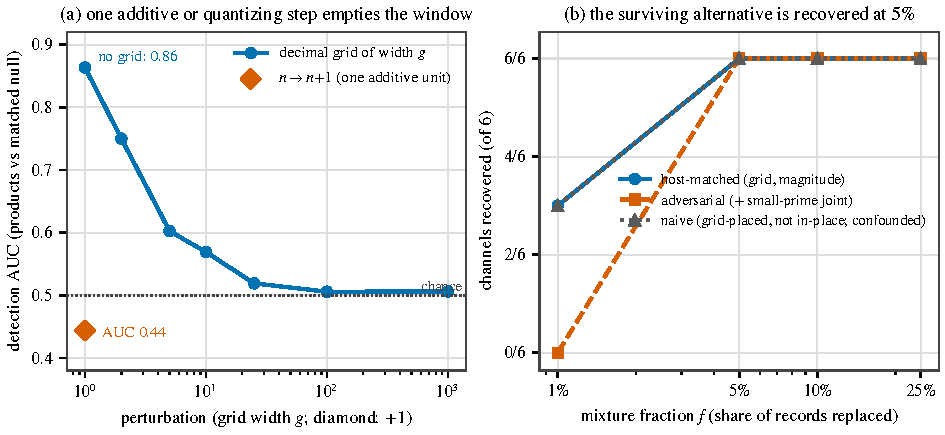
\includegraphics[width=\linewidth]{fig4_destruction_power}
\caption{Destruction and power. (a)~Detection AUC for exact composite
products under recording operations: grid coarsening degrades detection to
chance by width ${\sim}25$--$100$; one additive unit ($n \to n{+}1$, diamond)
collapses it below chance. (b)~Quotient-level spike-in: fraction of six real host channels recovered
versus mixture fraction, by injection tier. Both matched tiers are recovered
$6/6$ at $f = 0.05$; the confound check ($\max|z| < 3$) is clean in $6/6$
channels for the adversarial tier and $5/6$ for the host-matched tier
(Section~\ref{sec:power}).}
\label{fig:power}
\end{figure}

The result (Figure~\ref{fig:power}(b)): the host-matched tier is recovered in
six of six channels at a $5\%$ mixture (confound-clean in five; the one flag
is \emph{channel resonance}---residue-class concentration intrinsic to the
host's own values---which the injections dilute, not a grid leak), and the
adversarial tier is recovered six of six at $5\%$, confound-clean in all six.
The unit of detection deserves emphasis: ``recovered at $5\%$'' means the
\emph{channel-level} core statistic moves past the channel's own
$95$th-percentile noise band when one record in twenty is replaced---
population-level change detection, not identification of individual records.
The negative is therefore not underpowered \emph{against the model-implied
quotient-level multiplicative alternative in the tested host channels}: six
amount-kind channels here, and---in an exploratory v10.3 extension with its
plan frozen in advance---three count-kind hosts (telemetry byte counts, the
only count channels meeting the frozen magnitude screen), where the same
in-place injection is again recovered $3/3$ at a $5\%$ mixture. The extension's frozen rule reads, verbatim: ``count-host recovery HOLDS
iff $\ge$ half of hosts recovered at $f\le0.10$ with clean confound''
(clean $=\max|z|<3$); recovery is met, the confound condition is not, so
the extension does not qualify as clean recovery. In the count hosts the
mixture-level \emph{residue} coordinates drift below the host
($|z|$ $3.3$--$5.2$): the injections dilute the hosts' strong intrinsic
resonance, the same mechanism as the one flagged amount host, while the
decimal-grid coordinates stay within noise---so the flags mark dilution of
host structure, not grid leakage (supplement \S S5). When this pipeline
finds no residual in real channels, the evidence supports absence of
quotient-level multiplicative-history signal in the tested classes, not
absence of sensitivity.

Pre-registration covered this and every other confirmatory analysis: twenty
decision rules were frozen in configuration files before computation;
seventeen met their bars and three misfired. None of the misfires touches a
load-bearing conclusion---one retired a candidate whisper signal exactly as
its replicate-or-retire rule required, and two exposed miscalibrated secondary
statistics whose mechanical causes are instructive---and all three are
reported in full in the supplement rather than repaired.

\section{The instrument: measure the grid, not the shape}
\label{sec:instrument}

The boundary dictates the instrument. If the only multiplicative history a
recorded value retains is its grid, then a usable provenance readout should
measure the grid directly---and no per-record shape functional can do better,
since every one of them inherits the brittleness of
Section~\ref{sec:mechanism}. The recording-grid coordinates of
Section~\ref{sec:model} are that readout. Their demonstrated contribution is
precisely bounded: \emph{two real-data attribution instances, one constructed
detection case, and calibration contrasts}---not a general fabrication
detector.

\paragraph{Attribution instance 1: the CVAP false alarm.}
Section~\ref{sec:vignette} is the flagship. The coordinates attribute the
$\chi^2 = 12{,}684$ alarm to a five-grid: grid mass $0.275$ against $0.12$ for
enumerated votes, grid depth $0.55$, and residue excess $+0.77$ modulo $25$
($+0.73$ modulo $100$) against ${\approx}0$ for every enumerated series
(Figure~\ref{fig:cvap}(b)). The gate's own output is ``grid-compatible'';
it becomes an \emph{attribution} here because the Bureau's documentation
states the nearest-five rounding rule~\citep{cvaptechdoc}, closing the loop
from signature to mechanism. We claim an existence proof of the attribution
capability, not a generally validated procedure.

\paragraph{Attribution instance 2: the ACS margin-of-error localization.}
The American Community Survey provides the case where the instrument found
structure a digit analyst would not have tested~\citep{censusacs}. The
pre-registered expectation was that ACS county \emph{point estimates} would be
grid-marked relative to the decennial census. They are not (grid mass $0.107$
versus $0.112$; the frozen detection bar was missed and is reported as
missed). The publication grid lives instead in the \emph{margin-of-error}
column: grid mass $0.183$ ($90\%$ CI $[0.151, 0.216]$) against $0.112$
(Figure~\ref{fig:acs}). We have not located Census documentation stating a
margin-of-error rounding rule explicitly, so this instance is ``consistent
with a publication grid''---a localization, not a documentation-closed
attribution; CVAP remains the documented instance (the ACS technical
documentation~\citealp{acsstattest} describes the products generally). The
grid mark is subtle---partial rounding, visible to the CI-based grid-mass
comparison but below the coarse residue threshold of the validation library
in supplement \S S10. The two real instances differ usefully in kind: CVAP
is a false-alarm filter on the column an analyst does test; ACS is a localizer
pointing to a column nobody tests.

\begin{figure}[t]
\centering
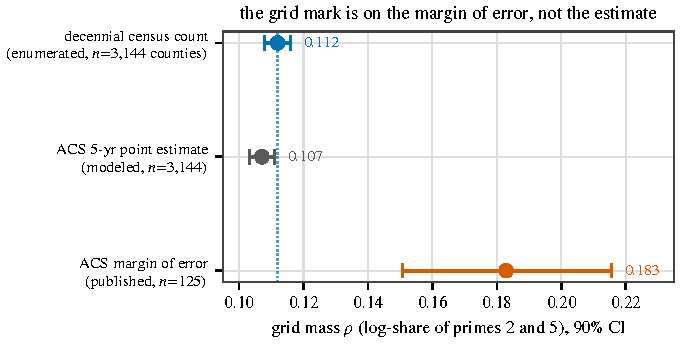
\includegraphics[width=0.72\linewidth]{fig5_acs_moe}
\caption{ACS margin-of-error localization: grid mass with $90\%$ bootstrap
intervals for county-level cross-sections. The modeled point estimate is not
grid-marked relative to the enumerated count (the pre-registered expectation
that it would be was wrong, and is reported as a miss); the published margin
of error is. The margin-of-error cross-section yields $125$ usable county
values under the frozen extraction screens; the estimate columns yield
$3{,}144$.}
\label{fig:acs}
\end{figure}

\paragraph{Bounded detection, and honest benchmarking.}
When the recording mechanism is a \emph{non-decimal} grid, the residue
coordinates can detect what terminal-digit tests cannot: on a constructed
contrast---real values re-quantized onto a $47$-tick versus a $43$-tick, both
invisible modulo $100$---the digit battery sits at or below AUC $0.53$ while
the residue coordinates read the tick at $1.00$. That is a scope
demonstration on constructed data, not real-world validation; no natural
non-decimal channel appeared in our corpus. On real returns the instrument
adds no detection value: read two-sided, a last-two-digit drift test reaches
AUC $1.00$ on the fabrication contrast and dominates the grid coordinates
($0.68$--$0.83$). We report the adverse comparison because omitting it would
be spin; the instrument's real-data role is attribution.

\paragraph{Calibration on two further quantities.}
Employment and votes calibrate the two axes on series of known provenance.
Survey employment estimates against the administrative near-census of the same
quantity: multiplicative axis null at every vintage ($\keff$ $0.98$--$1.00$),
survey hundreds-grid cleanly separated on the grid axis (grid mass $0.474$
versus $0.102$)~\citep{blsces,blsqcew}. Enumerated vote counts: $\keff$
$0.98$--$1.03$ at precinct, county, and state aggregation---additive tallies,
as expected---with residuals at trace scale ($+0.004$ to $+0.016$) appearing exactly where the
prospectively specified small-count caveat applies and absent elsewhere.
With population (ACS/decennial), the boundary is confirmed on three field
quantities (employment, population, votes); the fourth, byte counts, is
consistent---null at $\keff$ $0.996$ across $6{,}399$ telemetry count
channels, with the count-host power extension exploratory and its confound
bar not met (Section~\ref{sec:power}).

\paragraph{How a practitioner uses it.}
The demonstrated pattern is a two-step gate on a flagged field. First, run
whatever digit test raised the concern. If it fires, compute the grid
coordinates on the flagged partition against a clean reference. Elevated grid
mass, non-trivial grid depth, or residue excess at a modulus matching a
plausible tick attribute the alarm to a recording rule; their absence means
the anomaly is \emph{not} attributable to a grid this instrument can see, and
substantive investigation should proceed. The gate's output is always
``grid-compatible'' or ``not attributable to a visible grid''---never a
verdict on the data. A worked adversarial example makes this operational
(supplement \S S10): values \emph{fabricated} from a smooth generator and
then published on a five-grid fire the last-digit test
($\chi^2_9 \approx 11{,}800$) and the gate correctly reports
grid-compatible---because the alarm \emph{is} caused by the grid. The gate
attributes the alarm, not the data: it filters false positives; it never
certifies innocence.

\section{The complementary regime: exact integers}
\label{sec:exact}

The boundary is a statement about recorded data, not about the instrument's
intrinsic power, and the contrast deserves one compact section. Where integers
are exact, unrounded, produced by multiplication, and never subsequently
severed by addition or quantization, the shape window contains the whole
construction, and the profile is a working two-sided detector
(Figure~\ref{fig:exact}). On synthetic ground truth matched in magnitude and
moments: sums and Poisson tallies read $\keff = 1.00$ to two decimals
($0.997$--$0.998$), while products
of $k$ factors separate at AUC $0.86$--$0.96$. On genuine structured products
with closed-form factorizations (factorials, binomials, finite-group orders;
magnitudes to $10^{7263}$), all classes clear the pre-registered AUC bar of
$0.85$. On measured fields the detector reads both directions:
crystallographic multiplicity products at $\keff = 0.534 \pm 0.091$
($n = 11{,}240$), atomic degeneracy products at $1.707 \pm 0.557$ ($n = 505$),
graph automorphism orders (exact, to $10^{17{,}265}$) at $\keff$ up to
$4.44$---while real additive fields sit at $0.996$. This regime occurs by
construction in mathematics and the exact sciences and almost nowhere in
the administrative data classes tested here; the full catalogue, the balanced-pair edge case, and the
exact-arithmetic computation notes are in the supplement.

\begin{figure}[t]
\centering
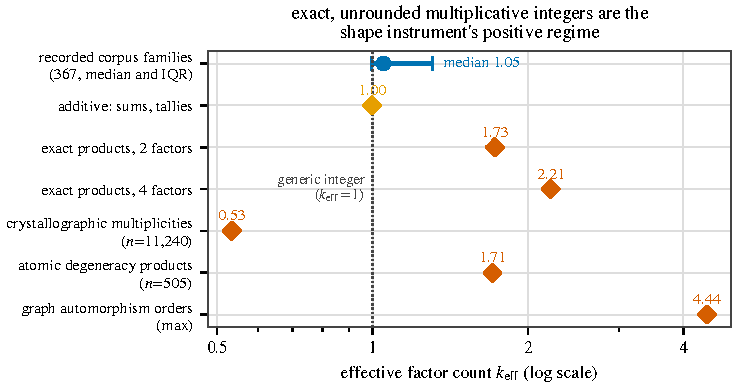
\includegraphics[width=0.78\linewidth]{fig6_exact_contrast}
\caption{The positive regime: effective factor count by class. Recorded
corpus families and additive constructions sit near the generic value
$\keff = 1$; exact multiplicative constructions and measured multiplicative
fields depart in both directions.}
\label{fig:exact}
\end{figure}

\section{Implications for data quality, forensic analysis, and audit}
\label{sec:implications}

The general lesson generalizes beyond factorization: a diagnostic reads only
what its projection encodes, and for recorded administrative integers---in the classes tested here---the
projection's window typically ends at the last recording operation. We
translate this into reporting practice.

A reported numerical anomaly on recorded data should state: the \emph{unit of
analysis} (record, channel, series); the \emph{scored population} (which
records survived screens); the \emph{representation} the detector reads
(digits, residues, factorization shape); the \emph{baseline} against which
``anomalous'' is defined (uniformity, magnitude-conditioned null, historical
control); any \emph{known recording or publication rule} for the series;
whether the result is \emph{detector-only} (a statistic fired),
\emph{statistically calibrated} (fired against a validated null), or
\emph{construction-attributed} (the responsible mechanism was identified);
the \emph{compatible alternative mechanisms}; and, explicitly, \emph{what
conclusion is licensed and what is not}.

\begin{table}[t]
\centering
\caption{The central warning, in usable form.}
\label{tab:warning}
\small
\begin{tabular}{p{0.44\linewidth}p{0.48\linewidth}}
\toprule
\multicolumn{2}{l}{\textbf{``Significant departure'' does not by itself mean:}} \\
\midrule
fabrication or misconduct & the rule that recorded the data can produce the same signature \\
risk or process change & the recording rule may have changed, not the process \\
data-quality failure & a documented publication grid is working as designed \\
\midrule
\multicolumn{2}{l}{\textbf{For a grid-attributed alarm, a valid conclusion is:}} \\
\midrule
\multicolumn{2}{p{0.94\linewidth}}{``The observed anomaly is consistent with,
and attributable to, a documented recording grid.''} \\
\midrule
\multicolumn{2}{l}{\textbf{It is not:}} \\
\midrule
\multicolumn{2}{p{0.94\linewidth}}{``The underlying records were
fabricated,'' or---equally---``the underlying records are genuine.''
Attribution of the alarm is not certification of the data.} \\
\bottomrule
\end{tabular}
\end{table}

Table~\ref{tab:warning} is the compact form, and supplement \S S10 turns it
into an operational protocol: the default modulus set and modal-grid recipe,
$z$-score and magnitude-matched-reference conventions, a multiplicity note,
stop/go criteria, the worked CVAP report with every field filled, the
fabricated-and-gridded adversarial example, and a ground-truth validation
library of seven grid-truth series (three documented real, four constructed)
and six non-grid series (sensitivity $6/7$, specificity $5/6$, both misses
mechanistically
explained: subtle partial rounding sits below the coarse threshold, and
small-magnitude series can false-flag---the same failure regime named in
Section~\ref{sec:mechanism}). In the CVAP case the licensed
conclusion is exactly the first: the alarm is attributable to the documented
five-grid. Nothing about the underlying tabulation's accuracy follows, in
either direction. The same discipline applies to the affirmative use of any
factorization-shape score on recorded data: a channel that looks
``anomalously composite'' or ``anomalously concentrated'' against a naive
reference is, in the classes tested here, exhibiting its magnitude and its
recording rule---as the deep-core episode of Section~\ref{sec:drivers} shows,
even a careful analysis can manufacture a survivor by mis-indexing the
reference.

For provenance practice, explicit lineage metadata---the W3C~PROV
model~\citep{provdm2013} and the provenance literature more
broadly~\citep{buneman2001,simmhan2005,cheney2009}---are strictly better
than inference from values where they exist. The grid coordinates are
a single-column profiling primitive in the tradition of automated data
profiling~\citep{abedjan2015,tane1999,metanome2015,hellerstein2008}, for the
common case where lineage is absent and the only witness is the stored
integers. The digit-forensics literature has long known that its tests can
mislead when recording assumptions fail~\citep{deckert2011,mebane2011,
klimek2012,lacasa2019}, and integer-percentage fingerprints of falsification
have their own electoral literature~\citep{kobak2016}; \citet{beberscacco2012} note that rounding must be
excluded for the last-digit test to be informative, but give no method. The
attribution gate is such a method for one class of mechanism.

\section{Limitations and conclusion}
\label{sec:limits}

\paragraph{Limitations, stated precisely and once.}
The boundary is a conditional empirical claim under
model~\eqref{eq:pipeline}, not a theorem; its completeness is an empirical
finding in one large but partly internal corpus dominated by a few
administrative sources. It concerns shape functionals of the log-share
multiset (blind to prime names given their sizes); named-prime instruments
are a different projection with a different boundary, and nothing here says
prime-specific arithmetic rules cannot survive recording. The powered null covers quotient-level composite
structure and balanced-pair mimics in six amount-kind host channels. The
attribution capability is demonstrated in two real instances, not validated
as a general method; the pre-specified gate is validated only on a small
ground-truth library (seven grid-truth series---three documented real, four
constructed---and six non-grid series; one miss each way, both explained); the non-decimal detection case is constructed, and
locating a natural coprime-tick channel is future work. The exact-integer results are
positive contrasts at demonstration scale. Field results cover three
statistical systems in one country. The new L1/L3 geography analyses are
exploratory (grouped-holdout design, family-level blocking, thresholds
declared in advance and labeled as project rules), and three pre-registered
predictions failed their frozen rules and are reported in the supplement. The
electoral material remains strictly methodological, as stated in
Section~\ref{sec:vignette}.

\paragraph{Conclusion.}
Factorization shape reads the accumulated multiplicative history since the
last additive or quantizing operation. For exact multiplicative integers, that
window can contain the whole construction; for ordinary recorded
administrative values---in the classes tested, under the stated recording
model---it is generally reduced to magnitude and the recording grid. A factorization-shape geography of recorded integers is therefore
usually a map of the recording pipeline, and the practical instrument the
boundary licenses reads the grid directly---which is exactly what turns a
catastrophic-looking digit alarm on a modeled population series into what it
was all along: a documented rounding rule, working as designed. The profile
reads the multiplicative history available after recording; for ordinary
administrative records, that history is often only the grid.

\section*{Data availability}
All analyzed series are public federal and state statistical products: BLS
Current Employment Statistics (archival real-time vintages)~\citep{blsces} and
Quarterly Census of Employment and Wages~\citep{blsqcew}; Census Bureau ACS
5-year estimates~\citep{censusacs}, decennial and Population Estimates Program
products, and the CVAP special tabulation~\citep{censuscvap2022}; North
Carolina State Board of Elections precinct returns~\citep{ncsbe} (the
certified-canvass primary source) and a community compilation of county-level
results assembled from state canvass pages and media
tabulations~\citep{countyreturns}, used as a calibration comparator; and, for
the exact-integer regime, the Crystallography Open Database~\citep{coddb}, the NIST
Atomic Spectra Database~\citep{nistasd}, and the SNAP network
collection~\citep{snap}. The frozen
configuration files, decision-rule manifest, per-claim manifest
(\texttt{claim\_manifest.csv}, mapping every numeric claim to script, output,
and SHA-256 hash), and hash-verified outputs are archived as a Zenodo deposit (DOI reserved;
an anonymized reviewer link is provided at submission), to be made public on
publication. The ``public products'' sentence above covers the field-calibration series;
the corpus's family-level access status (which source files are public,
which are hash-referenced local snapshots) is inventoried in the deposit.
The analysis uses only published aggregates, so the PRICSSA
checklist for complex-sample microdata analyses~\citep{seidenberg2023} does
not apply.
%% TODO(author): paste reserved-DOI + anonymized reviewer link at submission.

\section*{Code availability}
The analysis and figure code---extraction, exact factorization, grid
coordinates, spike-in, the exploratory geography build
(\texttt{stage22\_geo15.py}, with unit tests), and all figure scripts---is
version-controlled in a git repository [repository link at publication]. The
exact frozen state used for this manuscript (code, configuration files, the
decision-rule manifest, the claim manifest, and hash-verified outputs) is
archived as a Zenodo deposit (DOI reserved; anonymized reviewer link provided
at submission), with a worked end-to-end verification of the CVAP result in
the archive README. Repository and deposit will be made public on
publication.

\section*{Prospective specification}
Decision rules for all confirmatory analyses were prospectively specified in
internally frozen configuration files before computation ($20$ rules); this
is internal freezing with hash integrity, not external registry
timestamping (supplement \S S6). Three registered predictions failed
their frozen rules; they are reported, with mechanical causes, in the
supplement (\S S6). The L1/L3 geography analyses of
Sections~\ref{sec:geography} and~\ref{sec:mechanism} labeled ``exploratory''
were not covered by a frozen rule and are reported under the analysis plan
frozen in \texttt{run\_config\_geo15.json} before results were computed.

\bibliographystyle{plainnat}
\bibliography{references_v10}

\end{document}
